\documentclass[11pt]{article}
\usepackage[notes]{la}
\lamodule{4}{3}{Linearly Independent Sets; Bases}
\laxdoc{1.2}
\laxdoc{1.4}
\laxdoc{1.7}
\laxdoc{2.3}
\laxdoc{4.1}
\laxdoc{4.2}

\begin{document}

\section{Linearly Independent Sets; Bases}

\begin{guide}
In Section 4.2 every subspace we met came with a spanning set: free-variable vectors for $\Nul A$, columns for $\Col A$, rows for $\Row A$. But a spanning set can be wasteful. The columns of a matrix may repeat information, and a plane can be spanned by five vectors although two suffice. When is a spanning set \emph{wasteful}, and what exactly has been wasted? Is there a way to describe a subspace with no vector to spare, and how do we find such a description for the subspaces of a matrix, or for a subspace of polynomials, matrices or functions that is given by a condition?
\end{guide}

\textbf{By the end of this section you should be able to:}
\begin{itemize}
  \item decide whether a set of vectors in $\R^n$, in $\mathbb{P}_n$ or in $M_{2\times2}$ is linearly independent, by row reducing, and decide independence of functions by evaluating at well-chosen points;
  \item state and use the criterion ``a set of two or more vectors is dependent exactly when one of its vectors is a combination of the others'', and say when a vector may be removed without changing a span;
  \item define a \emph{basis} of a subspace, write down the standard bases of $\R^n$, $\mathbb{P}_n$ and $M_{2\times2}$, and decide, with a reason, whether a given set is a basis;
  \item state the Spanning Set Theorem and use it to shrink a spanning set to a basis;
  \item find a basis for $\Nul A$ (parametric vector form), for $\Col A$ (the pivot columns of $A$, \emph{not} of the echelon form) and for $\Row A$ (the nonzero rows of an echelon form), and explain why the columns of the echelon form are the wrong basis for $\Col A$;
  \item find a basis for a subspace described by an equation or a condition;
  \item describe a basis from two points of view: a spanning set from which nothing can be removed, and an independent set to which nothing can be added.
\end{itemize}

% ---------------------------------------------------------------------
\subsection*{Independence in a vector space}

In Section 1.7 a set of vectors of $\R^n$ was called linearly independent when the only combination that gives $\bv{0}$ is the trivial one (Definition~\ref{1.7-def:indep}). That definition uses nothing but the two operations of a vector space, adding vectors and multiplying them by scalars, together with the zero vector. So it makes sense word for word in any vector space from Section 4.1: polynomials, matrices, functions.

\begin{defn}{Linear independence in a vector space}{indepV}
Let $V$ be a vector space. An indexed set of vectors $\{\bv{v}_1,\dots,\bv{v}_p\}$ in $V$ is \emph{linearly independent} if the vector equation
\[
c_1\bv{v}_1+c_2\bv{v}_2+\cdots+c_p\bv{v}_p=\bv{0}
\]
has only the trivial solution $c_1=\cdots=c_p=0$. It is \emph{linearly dependent} if there are weights $c_1,\dots,c_p$, \emph{not all zero}, with $c_1\bv{v}_1+\cdots+c_p\bv{v}_p=\bv{0}$. Such an equation is a \emph{linear dependence relation}.
\end{defn}

Here $\bv{0}$ is the zero vector \emph{of $V$}: the zero polynomial, the zero matrix, the zero function. To test a set we must always do the same two things: write down the equation $c_1\bv{v}_1+\cdots+c_p\bv{v}_p=\bv{0}$ in $V$, and then decide whether the weights are forced to vanish. The first step looks different in each space; the second step is always a homogeneous system, which row reduction settles.

Three small cases need no work at all.

\begin{thm}{Small sets}{easy}
\begin{enumerate}[label=(\alph*),itemsep=1pt]
  \item A set $\{\bv{v}\}$ with a single vector is linearly independent if and only if $\bv{v}\neq\bv{0}$.
  \item A set that contains the zero vector is linearly dependent.
  \item A set of two vectors $\{\bv{u},\bv{v}\}$ is linearly dependent if and only if one of the vectors is a scalar multiple of the other.
\end{enumerate}
\end{thm}

\begin{proof}
(a)~If $\bv{v}\neq\bv{0}$ and $c\bv{v}=\bv{0}$, then $c=0$ (Theorem~\ref{4.1-thm:conseq}); and $1\cdot\bv{0}=\bv{0}$ is a dependence relation for $\{\bv{0}\}$. (b)~If $\bv{v}_1=\bv{0}$, then $1\cdot\bv{v}_1+0\cdot\bv{v}_2+\cdots+0\cdot\bv{v}_p=\bv{0}$ is a dependence relation. (c)~If $c_1\bv{u}+c_2\bv{v}=\bv{0}$ with $c_1\neq0$, then $\bv{u}=-\tfrac{c_2}{c_1}\bv{v}$; if $c_2\neq0$, then $\bv{v}=-\tfrac{c_1}{c_2}\bv{u}$. Conversely, $\bv{u}=k\bv{v}$ gives the relation $1\cdot\bv{u}-k\bv{v}=\bv{0}$.
\end{proof}

\subsubsection*{Vectors in $\R^n$}

For columns the test is Theorem~\ref{1.7-thm:cols}: put the vectors in a matrix and look for a pivot in every column.

\begin{exmp}{Columns that are dependent}{colsdep}
Are $\bv{v}_1=(1,0,2)$, $\bv{v}_2=(1,1,3)$ and $\bv{v}_3=(3,2,8)$ linearly independent?

\textbf{Solution.} The equation $x_1\bv{v}_1+x_2\bv{v}_2+x_3\bv{v}_3=\bv{0}$ is $A\bv{x}=\bv{0}$ for the matrix with these columns. Row reduce:
\begin{align*}
\begin{amat}{ccc}1&1&3\\0&1&2\\2&3&8\end{amat}
&\rops{R_3-2R_1}
\begin{amat}{ccc}1&1&3\\0&1&2\\0&1&2\end{amat}
\rops{R_3-R_2}
\begin{amat}{ccc}1&1&3\\0&1&2\\0&0&0\end{amat}
\\[4pt]
&\rops{R_1-R_2}
\begin{amat}{ccc}1&0&1\\0&1&2\\0&0&0\end{amat}
\end{align*}
Column $3$ has no pivot, so $x_3$ is free and there is a nonzero solution: $x_1=-x_3$ and $x_2=-2x_3$. Taking $x_3=1$,
\[
-\bv{v}_1-2\bv{v}_2+\bv{v}_3=\bv{0},\qquad\text{that is}\qquad \bv{v}_3=\bv{v}_1+2\bv{v}_2 .
\]
The set is linearly dependent, and the dependence relation says in which way: $(1,0,2)+2(1,1,3)=(3,2,8)$.
\end{exmp}

\begin{exmp}{Columns that are independent}{colsind}
Are $\bv{u}_1=(1,0,2,1)$, $\bv{u}_2=(0,1,1,-1)$ and $\bv{u}_3=(1,1,0,3)$ in $\R^4$ linearly independent?

\textbf{Solution.}
\begin{align*}
\begin{amat}{ccc}1&0&1\\0&1&1\\2&1&0\\1&-1&3\end{amat}
&\rops{R_3-2R_1}
\begin{amat}{ccc}1&0&1\\0&1&1\\0&1&-2\\1&-1&3\end{amat}
\rops{R_4-R_1}
\begin{amat}{ccc}1&0&1\\0&1&1\\0&1&-2\\0&-1&2\end{amat}
\\[4pt]
&\rops{R_3-R_2}
\begin{amat}{ccc}1&0&1\\0&1&1\\0&0&-3\\0&-1&2\end{amat}
\rops{R_4+R_2}
\begin{amat}{ccc}1&0&1\\0&1&1\\0&0&-3\\0&0&3\end{amat}
\\[4pt]
&\rops{R_4+R_3}
\begin{amat}{ccc}1&0&1\\0&1&1\\0&0&-3\\0&0&0\end{amat}
\end{align*}
Every column has a pivot (the last row has become a row of zeros), so $A\bv{x}=\bv{0}$ has only the trivial solution: the set is linearly independent. Notice that a pivot in every \emph{column} is what matters here; there is no need for a pivot in every row, and with four rows and three columns there cannot be one.
\end{exmp}

\begin{exmp}{A parameter}{param}
For which values of $h$ are $\bv{v}_1=(1,2,0)$, $\bv{v}_2=(2,5,3)$ and $\bv{v}_3=(1,3,h)$ linearly dependent?

\textbf{Solution.} Keep $h$ in the matrix and reduce:
\begin{align*}
\begin{amat}{ccc}1&2&1\\2&5&3\\0&3&h\end{amat}
&\rops{R_2-2R_1}
\begin{amat}{ccc}1&2&1\\0&1&1\\0&3&h\end{amat}
\rops{R_3-3R_2}
\begin{amat}{ccc}1&2&1\\0&1&1\\0&0&h - 3\end{amat}
\end{align*}
The first two columns always have pivots. The third column has a pivot exactly when $h-3\neq0$. So the set is dependent only for $h=3$, and independent for every other $h$. For $h=3$ the relation is found by continuing: $x_3$ is free, $x_2=-x_3$, $x_1=x_3$, so $\bv{v}_1-\bv{v}_2+\bv{v}_3=\bv{0}$; check: $(1,2,0)-(2,5,3)+(1,3,3)=(0,0,0)$.
\end{exmp}

\begin{kc}{Test the columns}{cols}
Row reduce to decide whether each set is linearly independent. If it is dependent, write down a dependence relation. (a)~$(1,-1,2),\ (2,0,1),\ (3,-3,4)$ in $\R^3$. (b)~$(1,3),\ (2,7)$ in $\R^2$. (c)~$(1,0,1,0),\ (0,1,0,1),\ (1,1,1,1)$ in $\R^4$. (d)~$(1,2),\ (3,1),\ (4,3)$ in $\R^2$.
\end{kc}

\subsubsection*{Polynomials and matrices}

In $\mathbb{P}_n$ the equation $c_1p_1+\cdots+c_pp_p=\bv{0}$ says that a polynomial is the zero polynomial, and a polynomial is zero when \emph{all its coefficients are zero}. So we collect the coefficients of $1,t,t^2,\dots$ and obtain one linear equation for each power of $t$. In $M_{2\times2}$ a matrix is zero when all four entries are zero, which gives four equations. In both cases the unknowns are the weights $c_1,\dots,c_p$, and the coefficient matrix has one column for each vector.

\begin{exmp}{Polynomials in $\mathbb{P}_2$}{polys}
\textbf{(a)} Let $p_1=1+2t$, $p_2=t+t^2$, $p_3=1-t^2$. The equation $c_1p_1+c_2p_2+c_3p_3=\bv{0}$ means
\[
(c_1+c_3)+(2c_1+c_2)t+(c_2-c_3)t^2=0\quad\text{for all }t,\qquad\text{so}\qquad c_1+c_3=0,\ \ 2c_1+c_2=0,\ \ c_2-c_3=0.
\]
The coefficient matrix has the weights of $1$, $t$, $t^2$ in its rows and one column for each polynomial:
\begin{align*}
\begin{amat}{ccc}1&0&1\\2&1&0\\0&1&-1\end{amat}
&\rops{R_2-2R_1}
\begin{amat}{ccc}1&0&1\\0&1&-2\\0&1&-1\end{amat}
\rops{R_3-R_2}
\begin{amat}{ccc}1&0&1\\0&1&-2\\0&0&1\end{amat}
\end{align*}
Three pivots, one in each column: only $c_1=c_2=c_3=0$ solves the system, so $\{p_1,p_2,p_3\}$ is linearly independent.

\textbf{(b)} Change the last polynomial to $q_3=1-t^2$ and the first to $q_1=1+t$, and take $q_2=t+t^2$:
\begin{align*}
\begin{amat}{ccc}1&0&1\\1&1&0\\0&1&-1\end{amat}
&\rops{R_2-R_1}
\begin{amat}{ccc}1&0&1\\0&1&-1\\0&1&-1\end{amat}
\rops{R_3-R_2}
\begin{amat}{ccc}1&0&1\\0&1&-1\\0&0&0\end{amat}
\end{align*}
Now the third column is free: $c_3=1$ gives $c_2=1$ and $c_1=-1$, and indeed $-(1+t)+(t+t^2)+(1-t^2)=0$. The set $\{1+t,\ t+t^2,\ 1-t^2\}$ is linearly dependent, and $1-t^2=(1+t)-(t+t^2)$.
\end{exmp}

\begin{exmp}{Matrices in $M_{2\times2}$}{mats}
Let $M_1=\begin{bmatrix}1&1\\0&0\end{bmatrix}$, \ $M_2=\begin{bmatrix}0&1\\1&0\end{bmatrix}$, \ $M_3=\begin{bmatrix}0&0\\1&1\end{bmatrix}$ and $I=\begin{bmatrix}1&0\\0&1\end{bmatrix}$. Then
\[
c_1M_1+c_2M_2+c_3M_3=\begin{bmatrix}c_1&c_1+c_2\\c_2+c_3&c_3\end{bmatrix},
\]
which is the zero matrix only if $c_1=0$, $c_3=0$ and then $c_2=0$. So $\{M_1,M_2,M_3\}$ is linearly independent. Adding $I$ changes the answer: $c_1M_1+c_2M_2+c_3M_3+c_4I=\bv{0}$ means $c_1+c_4=0$, $c_1+c_2=0$, $c_2+c_3=0$, $c_3+c_4=0$ (the four entries in the order $a_{11},a_{12},a_{21},a_{22}$), and
\begin{align*}
\begin{amat}{cccc}1&0&0&1\\1&1&0&0\\0&1&1&0\\0&0&1&1\end{amat}
&\rops{R_2-R_1}
\begin{amat}{cccc}1&0&0&1\\0&1&0&-1\\0&1&1&0\\0&0&1&1\end{amat}
\rops{R_3-R_2}
\begin{amat}{cccc}1&0&0&1\\0&1&0&-1\\0&0&1&1\\0&0&1&1\end{amat}
\\[4pt]
&\rops{R_4-R_3}
\begin{amat}{cccc}1&0&0&1\\0&1&0&-1\\0&0&1&1\\0&0&0&0\end{amat}
\end{align*}
has a free fourth column. With $c_4=1$ we get $c_3=-1$, $c_2=1$, $c_1=-1$:
\[
-M_1+M_2-M_3+I=\mathbf{0},\qquad\text{that is}\qquad I=M_1-M_2+M_3 .
\]
Check: $\begin{bmatrix}1&1\\0&0\end{bmatrix}-\begin{bmatrix}0&1\\1&0\end{bmatrix}+\begin{bmatrix}0&0\\1&1\end{bmatrix}=\begin{bmatrix}1&0\\0&1\end{bmatrix}$. The set $\{M_1,M_2,M_3,I\}$ is linearly dependent.
\end{exmp}

\begin{kc}{Polynomials and matrices}{polymat}
Decide whether each set is linearly independent, and if not find a dependence relation. (a)~$2+t,\ 1+t^2,\ t+t^2$ in $\mathbb{P}_2$. (b)~$1+t,\ t+t^2,\ t^2+t^3,\ 1+t^3$ in $\mathbb{P}_3$. (c)~$\begin{bmatrix}1&2\\0&1\end{bmatrix},\ \begin{bmatrix}0&1\\1&1\end{bmatrix},\ \begin{bmatrix}1&0\\-2&-1\end{bmatrix}$ in $M_{2\times2}$.
\end{kc}

\subsubsection*{Functions}

A set of functions $f_1,\dots,f_p$ on an interval is independent if $c_1f_1+\cdots+c_pf_p$ equals the \emph{zero function}, meaning that it is $0$ at \emph{every} input, only for $c_1=\cdots=c_p=0$ (Example~\ref{4.1-ex:functions}). If the combination is zero for all $t$, it is in particular zero at any $t$ we choose. That gives us equations to work with: \emph{evaluate at points}.

\begin{exmp}{$\sin t$ and $\cos t$}{sincos}
Suppose $c_1\sin t+c_2\cos t=0$ for every $t$. Put $t=0$: $c_1\cdot0+c_2\cdot1=0$, so $c_2=0$. Put $t=\tfrac{\pi}{2}$: $c_1\cdot1+c_2\cdot0=0$, so $c_1=0$. Only the trivial combination vanishes, so $\{\sin t,\cos t\}$ is linearly independent. (Neither function is a constant multiple of the other: Theorem~\ref{thm:easy}(c) gives a second reason, but the evaluation argument is the one that generalises.)
\end{exmp}

\begin{exmp}{More functions}{moreF}
\textbf{(a)} $\{1,\ t,\ t^2\}$ as functions on $\R$. If $c_1+c_2t+c_3t^2=0$ for all $t$, then at $t=0,1,-1$:
\[
\begin{bmatrix}1&0&0\\1&1&1\\1&-1&1\end{bmatrix}\begin{bmatrix}c_1\\c_2\\c_3\end{bmatrix}=\begin{bmatrix}0\\0\\0\end{bmatrix}.
\]
The matrix is invertible (its determinant is $2$; or row reduce), so $c_1=c_2=c_3=0$: the three functions are independent.

\textbf{(b)} $\{e^t,\ e^{2t}\}$. At $t=0$ and $t=\ln2$ the values are $(1,1)$ and $(2,4)$, so
$\begin{bmatrix}1&1\\2&4\end{bmatrix}\begin{bmatrix}c_1\\c_2\end{bmatrix}=\begin{bmatrix}0\\0\end{bmatrix}$ has only the trivial solution (determinant $2$): independent.

\textbf{(c)} $\{\sin t,\ \cos t,\ \sin(t+\tfrac{\pi}{3})\}$. The addition formula gives $\sin(t+\tfrac{\pi}{3})=\tfrac12\sin t+\tfrac{\sqrt3}{2}\cos t$ for all $t$, so
\[
\tfrac12\sin t+\tfrac{\sqrt3}{2}\cos t-\sin(t+\tfrac{\pi}{3})=0
\]
is a dependence relation: the set is dependent. No choice of points could have shown this directly (see the warning below).

\textbf{(d)} $\{1,\ \cos2t,\ \cos^2t\}$ is dependent, because $\cos2t=2\cos^2t-1$ for all $t$: $\ 1+\cos2t-2\cos^2t=0$.
\end{exmp}

\begin{warn}[Evaluating at points can prove independence only]
If a combination $c_1f_1+\cdots+c_pf_p$ is the zero function, then it vanishes at every point, in particular at the points you choose. So if the equations at \emph{some} points already force all $c_j=0$, the set is independent (Examples~\ref{ex:sincos} and~\ref{ex:moreF}(a),(b)). But if the equations you get have a nonzero solution, you have learned nothing yet: the combination might vanish at your points and not at others. To prove dependence you must show that a combination is zero at \emph{every} input, as the identities in Example~\ref{ex:moreF}(c),(d) do.
\end{warn}

\begin{kc}{Independent functions?}{funcs}
(a)~Show that $\{1,\ e^t\}$ is linearly independent by evaluating at $t=0$ and $t=1$. (b)~Show that $\{\cos t,\ \cos2t\}$ is independent by evaluating at $t=0$ and $t=\tfrac{\pi}{2}$. (c)~Is $\{\sin2t,\ \sin t\cos t\}$ independent? Evaluate at $t=0$ and at $t=\tfrac{\pi}{4}$; what do the equations say, and what does the identity $\sin2t=2\sin t\cos t$ say?
\end{kc}

\begin{think}{Why the zero vector ruins independence}{zerovec}
(a)~Without computing, explain why $\{\bv{0},\bv{v}\}$ is dependent for every $\bv{v}$ (Theorem~\ref{thm:easy}(b)). (b)~Is the one-element set $\{\bv{0}\}$ dependent? (c)~A matrix has a column of zeros. What does Theorem~\ref{1.7-thm:cols} say about the columns, and which free variable shows it?
\end{think}

\begin{think}{Evaluating at points}{evalpts}
(a)~To show that $\{1,t,t^2\}$ is independent we evaluated at three points. Would two points have been enough? Would the points $t=1,2,3$ have worked equally well? (b)~In Example~\ref{ex:moreF}(d) try the points $t=0$ and $t=\tfrac{\pi}{2}$. Does the system of equations for $c_1,c_2,c_3$ have a nonzero solution? Does that prove dependence?
\end{think}

% ---------------------------------------------------------------------
\subsection*{Dependence means redundancy}

When a set is dependent, a dependence relation with a nonzero weight can be solved for the corresponding vector. That is the content of the following criterion, which in $\R^n$ is Theorem~\ref{1.7-thm:char}. The proof works in every vector space.

\begin{thm}{The dependence-relation criterion}{criterion}
Let $S=\{\bv{v}_1,\dots,\bv{v}_p\}$ be a set of two or more vectors in a vector space $V$.
\begin{enumerate}[label=(\alph*),itemsep=1pt]
  \item $S$ is linearly dependent if and only if at least one of the vectors is a linear combination of the others. In that case that vector can be removed without changing $\Span S$.
  \item If $\bv{v}_1\neq\bv{0}$, then $S$ is linearly dependent if and only if some $\bv{v}_j$ with $j\ge2$ is a linear combination of the \emph{preceding} vectors $\bv{v}_1,\dots,\bv{v}_{j-1}$.
\end{enumerate}
\end{thm}

\begin{proof}
(a)~Suppose $c_1\bv{v}_1+\cdots+c_p\bv{v}_p=\bv{0}$ with $c_k\neq0$ for some $k$. Solving for $\bv{v}_k$,
\[
\bv{v}_k=-\tfrac{c_1}{c_k}\bv{v}_1-\cdots-\tfrac{c_p}{c_k}\bv{v}_p\quad(\text{the term with }\bv{v}_k\text{ left out}),
\]
so $\bv{v}_k$ is a combination of the others. Conversely, if $\bv{v}_k=a_1\bv{v}_1+\cdots+a_p\bv{v}_p$ (without $\bv{v}_k$ on the right), then $a_1\bv{v}_1+\cdots-1\cdot\bv{v}_k+\cdots+a_p\bv{v}_p=\bv{0}$ is a dependence relation, since the weight of $\bv{v}_k$ is $-1\neq0$. For the last sentence: any combination of $\bv{v}_1,\dots,\bv{v}_p$ that uses $\bv{v}_k$ can be rewritten by substituting the expression for $\bv{v}_k$, which gives a combination of the others with the same value.

(b)~If $\bv{v}_j$ is a combination of the preceding vectors, then $S$ is dependent by (a). Conversely, let $c_1\bv{v}_1+\cdots+c_p\bv{v}_p=\bv{0}$ with not all weights zero, and let $j$ be the \emph{largest} index with $c_j\neq0$. If $j=1$, then $c_1\bv{v}_1=\bv{0}$ with $c_1\neq0$ forces $\bv{v}_1=\bv{0}$, contrary to the hypothesis. So $j\ge2$, and the terms after $j$ vanish: $c_1\bv{v}_1+\cdots+c_j\bv{v}_j=\bv{0}$. Solving for $\bv{v}_j$ expresses it through $\bv{v}_1,\dots,\bv{v}_{j-1}$.
\end{proof}

\begin{warn}[One of the vectors not every vector]
The criterion says that \emph{at least one} vector is a combination of the others, not that every vector is. In $\{(1,0),(2,0),(0,1)\}$ the first two vectors are multiples of each other, so the set is dependent, but $(0,1)$ is not a combination of $(1,0)$ and $(2,0)$. Removing $(0,1)$ would change the span. Removing $(1,0)$ or $(2,0)$ would not. A dependence relation tells you which vectors are redundant: those with a \emph{nonzero} weight.
\end{warn}

\begin{exmp}{Which vector is redundant?}{redundant}
Let $\bv{w}_1=(1,0,2)$, $\bv{w}_2=(0,1,-1)$ and $\bv{w}_3=(2,3,1)$. Find a dependence relation and express each vector as a combination of the others.

\textbf{Solution.}
\begin{align*}
\begin{amat}{ccc}1&0&2\\0&1&3\\2&-1&1\end{amat}
&\rops{R_3-2R_1}
\begin{amat}{ccc}1&0&2\\0&1&3\\0&-1&-3\end{amat}
\rops{R_3+R_2}
\begin{amat}{ccc}1&0&2\\0&1&3\\0&0&0\end{amat}
\end{align*}
Column $3$ is free: $x_1=-2x_3$ and $x_2=-3x_3$, so $-2\bv{w}_1-3\bv{w}_2+\bv{w}_3=\bv{0}$. All three weights are nonzero, so \emph{each} vector is a combination of the other two:
\[
\bv{w}_3=2\bv{w}_1+3\bv{w}_2,\qquad \bv{w}_1=-\tfrac32\bv{w}_2+\tfrac12\bv{w}_3,\qquad \bv{w}_2=-\tfrac23\bv{w}_1+\tfrac13\bv{w}_3 .
\]
Check the first: $2(1,0,2)+3(0,1,-1)=(2,3,1)$. Any one of the three can be removed; the other two still span the same plane.
\end{exmp}

\begin{exmp}{The preceding-vector version, and why the order matters}{preceding}
Let $\bv{v}_1=(1,2)$, $\bv{v}_2=(0,1)$ and $\bv{v}_3=(1,3)$. Here $\bv{v}_3=\bv{v}_1+\bv{v}_2$ is a combination of the preceding vectors, as Theorem~\ref{thm:criterion}(b) promises (the set is dependent because three vectors in $\R^2$ cannot be independent, Theorem~\ref{1.7-thm:count}). But also $\bv{v}_1=\bv{v}_3-\bv{v}_2$ is a combination of the \emph{other} vectors; it is not a combination of the preceding ones, because there are none. List the same vectors as $\bv{v}_3,\bv{v}_2,\bv{v}_1$: now the third vector $\bv{v}_1=\bv{v}_3-\bv{v}_2$ is a combination of the preceding two. The set is the same; only the order changed, and with it the vector that statement (b) points to. Part~(a) does not care about order, part~(b) does.
\end{exmp}

\begin{exmp}{Redundancy by inspection}{inspect}
Decide at a glance which sets are dependent, and why.

\textbf{(a)} $\{(1,2,3),\ (0,0,0),\ (4,1,1)\}$: contains $\bv{0}$ (Theorem~\ref{thm:easy}(b)). Dependent.

\textbf{(b)} $\{(1,-2,3),\ (-3,6,-9)\}$: the second vector is $-3$ times the first (Theorem~\ref{thm:easy}(c)). Dependent.

\textbf{(c)} $\{(1,2,3),\ (2,1,0),\ (0,1,1),\ (5,5,5)\}$: four vectors in $\R^3$ (Theorem~\ref{1.7-thm:count}). Dependent.

\textbf{(d)} $\{1,\ 1+t,\ 2-3t\}$ in $\mathbb{P}_1$: three vectors in a space of polynomials $a_0+a_1t$ that are determined by two numbers. Dependent (write it as three columns in $\R^2$).

\textbf{(e)} $\{(1,2),\ (3,4)\}$: two vectors, neither a multiple of the other. Independent (Theorem~\ref{thm:easy}(c)).

\textbf{(f)} $\{(1,0,0),\ (0,1,0),\ (1,1,1)\}$: no vector is a combination of the others, since the third has a nonzero third entry and the first two have none. A dependence relation would need weight $0$ on the third vector, then on the other two. Independent.
\end{exmp}

\begin{center}
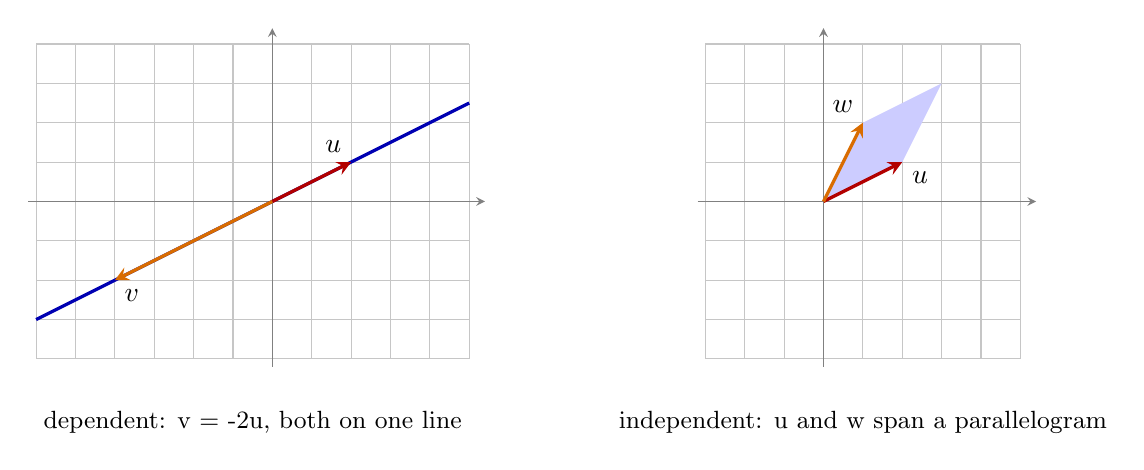
\begin{tikzpicture}[x=0.5cm,y=0.5cm,>=stealth]
  \draw[gray!45] (-6,-4) grid[step=1] (5,4);
  \draw[->,gray] (-6.2,0)--(5.4,0);
  \draw[->,gray] (0,-4.2)--(0,4.4);
  \draw[very thick,blue!70!black] (-6,-3)--(5,2.5);
  \draw[->,very thick,red!70!black] (0,0)--(2,1);
  \draw[->,very thick,orange!85!black] (0,0)--(-4,-2);
  \node[above left] at (2,1) {$u$};
  \node[below right] at (-4,-2) {$v$};
  \node at (-0.5,-5.6) {\small dependent: v = -2u, both on one line};
  \begin{scope}[shift={(14,0)}]
    \draw[gray!45] (-3,-4) grid[step=1] (5,4);
    \draw[->,gray] (-3.2,0)--(5.4,0);
    \draw[->,gray] (0,-4.2)--(0,4.4);
    \fill[blue!20] (0,0)--(2,1)--(3,3)--(1,2)--cycle;
    \draw[->,very thick,red!70!black] (0,0)--(2,1);
    \draw[->,very thick,orange!85!black] (0,0)--(1,2);
    \node[below right] at (2,1) {$u$};
    \node[above left] at (1,2) {$w$};
    \node at (1,-5.6) {\small independent: u and w span a parallelogram};
  \end{scope}
\end{tikzpicture}
\end{center}

\textbf{Figure 1.} Left: $\bv{u}=(2,1)$ and $\bv{v}=(-4,-2)=-2\bv{u}$. Both lie on one line through the origin, so $\Span\{\bv{u},\bv{v}\}$ is that line and the relation $2\bv{u}+\bv{v}=\bv{0}$ holds. Right: $\bv{u}=(2,1)$ and $\bv{w}=(1,2)$ point in different directions. The parallelogram they span has positive area, nothing collapses, and the only combination $c_1\bv{u}+c_2\bv{w}$ equal to $\bv{0}$ is the trivial one. (Its area is $|2\cdot2-1\cdot1|=3$.)

\begin{kc}{Which vectors may be removed?}{removable}
Let $\bv{u}_1=(1,1,0)$, $\bv{u}_2=(0,1,1)$, $\bv{u}_3=(1,2,1)$ and $\bv{u}_4=(0,0,1)$. (a)~Show that $\bv{u}_3=\bv{u}_1+\bv{u}_2$. (b)~Which of the four vectors can be removed without changing the span, and which cannot? (c)~Is the set $\{\bv{u}_1,\bv{u}_2,\bv{u}_3,\bv{u}_4\}$ linearly dependent?
\end{kc}

\begin{think}{Order and the preceding vectors}{order}
(a)~In Example~\ref{ex:preceding}, why could $\bv{v}_1$ not be written as a combination of the preceding vectors? What does that say about the hypothesis $\bv{v}_1\neq\bv{0}$ in Theorem~\ref{thm:criterion}(b)? (b)~Take $\bv{v}_1=\bv{0}$ and $\bv{v}_2=(1,0)$. Is $\{\bv{v}_1,\bv{v}_2\}$ dependent? Is $\bv{v}_2$ a combination of the preceding vector $\bv{v}_1$? What does this show about the hypothesis $\bv{v}_1\neq\bv{0}$?
\end{think}

% ---------------------------------------------------------------------
\subsection*{Bases}

A spanning set describes a subspace; an independent set wastes nothing. A set with both properties is the efficient description we were looking for.

\begin{defn}{Basis}{basis}
Let $H$ be a subspace of a vector space $V$. An indexed set of vectors $\mathcal{B}=\{\bv{b}_1,\dots,\bv{b}_p\}$ in $H$ is a \emph{basis for $H$} if
\begin{enumerate}[label=(\roman*),itemsep=1pt]
  \item $\mathcal{B}$ is a linearly independent set, and
  \item $\mathcal{B}$ spans $H$, that is, $\Span\mathcal{B}=H$.
\end{enumerate}
Since $V$ is a subspace of itself, the definition also tells what a basis for $V$ is.
\end{defn}

Both parts matter: a spanning set that is not independent has a vector to spare, and an independent set that does not span leaves part of $H$ out. A subspace has many bases, as we shall see; ``a basis for $H$'' and ``the basis'' are different things.

\begin{exmp}{The standard bases}{standard}
\textbf{(a) $\R^n$.} The columns $\bv{e}_1,\dots,\bv{e}_n$ of the identity matrix (Example~\ref{1.4-ex:ei}) are the \emph{standard basis} of $\R^n$. They span, since $(x_1,\dots,x_n)=x_1\bv{e}_1+\cdots+x_n\bv{e}_n$, and they are independent, since the identity matrix has a pivot in every column. For $\R^3$: $\bv{e}_1=(1,0,0)$, $\bv{e}_2=(0,1,0)$, $\bv{e}_3=(0,0,1)$.

\textbf{(b) $\mathbb{P}_n$.} The polynomials $1,t,t^2,\dots,t^n$ form the \emph{standard basis} of $\mathbb{P}_n$. They span, since every polynomial of degree at most $n$ is $a_0\cdot1+a_1t+\cdots+a_nt^n$ by the very definition of $\mathbb{P}_n$. They are independent: a combination $c_0+c_1t+\cdots+c_nt^n$ is the zero polynomial only if all its coefficients are zero. For $\mathbb{P}_2$: $\{1,t,t^2\}$.

\textbf{(c) $M_{2\times2}$.} Let $E_{11}=\begin{bmatrix}1&0\\0&0\end{bmatrix}$, $E_{12}=\begin{bmatrix}0&1\\0&0\end{bmatrix}$, $E_{21}=\begin{bmatrix}0&0\\1&0\end{bmatrix}$ and $E_{22}=\begin{bmatrix}0&0\\0&1\end{bmatrix}$. Then
\[
\begin{bmatrix}a&b\\c&d\end{bmatrix}=aE_{11}+bE_{12}+cE_{21}+dE_{22},
\]
so $\{E_{11},E_{12},E_{21},E_{22}\}$ spans $M_{2\times2}$; and the combination on the right is the zero matrix only if $a=b=c=d=0$, so the set is independent. It is the \emph{standard basis} of $M_{2\times2}$.
\end{exmp}

For a set of $n$ vectors in $\R^n$ the Invertible Matrix Theorem (Theorem~\ref{2.3-thm:imt}) answers both questions in one stroke: with $n$ columns and $n$ rows, ``independent'' (a pivot in every column), ``spanning'' (a pivot in every row) and ``invertible'' are one statement.

\begin{exmp}{Is it a basis? Reasons}{isbasis}
\textbf{(a)} $\mathcal{B}=\{(1,1,0),\ (0,1,1),\ (1,0,1)\}$ in $\R^3$. These are the columns of a $3\times3$ matrix:
\begin{align*}
\begin{amat}{ccc}1&0&1\\1&1&0\\0&1&1\end{amat}
&\rops{R_2-R_1}
\begin{amat}{ccc}1&0&1\\0&1&-1\\0&1&1\end{amat}
\rops{R_3-R_2}
\begin{amat}{ccc}1&0&1\\0&1&-1\\0&0&2\end{amat}
\end{align*}
Three pivots: the matrix is invertible, so the columns are independent \emph{and} span $\R^3$ (Theorem~\ref{2.3-thm:imt}). Yes, a basis for $\R^3$.

\textbf{(b)} $\{(1,2,3),\ (0,1,1)\}$ in $\R^3$. The two vectors are not multiples of each other, so the set is independent (Theorem~\ref{thm:easy}(c)). But two vectors have only two pivots at most, while $\R^3$ has three rows, so the set does not span $\R^3$: for instance $(1,0,0)$ is not a combination (the equation $x_1(1,2,3)+x_2(0,1,1)=(1,0,0)$ gives $x_1=1$, $x_2=-2$ and then $3-2=1\neq0$). \emph{Not} a basis for $\R^3$. It \emph{is} a basis for the plane $H=\Span\{(1,2,3),(0,1,1)\}$ that it spans.

\textbf{(c)} $\{(1,0,0),\ (0,1,0),\ (0,0,1),\ (1,1,1)\}$ in $\R^3$. It spans $\R^3$ (it contains the standard basis) but it is dependent: $(1,1,1)=\bv{e}_1+\bv{e}_2+\bv{e}_3$. Not a basis.

\textbf{(d)} $\{1,\ t,\ 1+t\}$ in $\mathbb{P}_2$. Dependent ($1+t$ is the sum of the other two) and it does not span $\mathbb{P}_2$ either, since no combination has a $t^2$ term. Not a basis for $\mathbb{P}_2$; it spans $\mathbb{P}_1$ but is not a basis of that either, because it is dependent.
\end{exmp}

\begin{exmp}{A basis of $\mathbb{P}_2$ that is not the standard one}{polybasis}
Let $\mathcal{B}=\{1,\ 1+t,\ 1+t+t^2\}$. \emph{Independent:} $c_1+c_2(1+t)+c_3(1+t+t^2)=(c_1+c_2+c_3)+(c_2+c_3)t+c_3t^2=0$ forces $c_3=0$, then $c_2=0$, then $c_1=0$. \emph{Spanning:} given $a_0+a_1t+a_2t^2$ we solve the same triangular system backwards, $c_3=a_2$, $c_2=a_1-a_2$, $c_1=a_0-a_1$, and indeed
\[
(a_0-a_1)\cdot1+(a_1-a_2)(1+t)+a_2(1+t+t^2)=a_0+a_1t+a_2t^2 .
\]
So $\mathcal{B}$ is a basis for $\mathbb{P}_2$. For example, for $2-3t+5t^2$ the weights are $c_3=5$, $c_2=-3-5=-8$, $c_1=2+3=5$, and $5\cdot1-8(1+t)+5(1+t+t^2)=(5-8+5)+(-8+5)t+5t^2=2-3t+5t^2$.
\end{exmp}

\begin{exmp}{A basis of $M_{2\times2}$ made of unusual matrices}{matbasis}
Let $I=\begin{bmatrix}1&0\\0&1\end{bmatrix}$, $S=\begin{bmatrix}0&1\\1&0\end{bmatrix}$, $Z=\begin{bmatrix}1&0\\0&-1\end{bmatrix}$ and $J=\begin{bmatrix}0&1\\-1&0\end{bmatrix}$. Is $\{I,S,Z,J\}$ a basis for $M_{2\times2}$?

\textbf{Solution.} Write each matrix as the list $(a_{11},a_{12},a_{21},a_{22})$ of its entries. The four lists are $(1,0,0,1)$, $(0,1,1,0)$, $(1,0,0,-1)$, $(0,1,-1,0)$; as the columns of a $4\times4$ matrix:
\begin{align*}
\begin{amat}{cccc}1&0&1&0\\0&1&0&1\\0&1&0&-1\\1&0&-1&0\end{amat}
&\rops{R_4-R_1}
\begin{amat}{cccc}1&0&1&0\\0&1&0&1\\0&1&0&-1\\0&0&-2&0\end{amat}
\rops{R_3-R_2}
\begin{amat}{cccc}1&0&1&0\\0&1&0&1\\0&0&0&-2\\0&0&-2&0\end{amat}
\\[4pt]
&\rops{R_3\leftrightarrow R_4}
\begin{amat}{cccc}1&0&1&0\\0&1&0&1\\0&0&-2&0\\0&0&0&-2\end{amat}
\end{align*}
Four pivots in four columns and four rows: independent \emph{and} spanning. It is a basis, and it even gives a recipe: solving for the weights of $\begin{bmatrix}a&b\\c&d\end{bmatrix}$,
\[
\begin{bmatrix}a&b\\c&d\end{bmatrix}=\tfrac{a+d}{2}I+\tfrac{b+c}{2}S+\tfrac{a-d}{2}Z+\tfrac{b-c}{2}J .
\]
Check with $\begin{bmatrix}1&2\\3&4\end{bmatrix}$: the weights are $\tfrac52,\tfrac52,-\tfrac32,-\tfrac12$, and the four entries of the combination are $\tfrac52-\tfrac32=1$, \ $\tfrac52-\tfrac12=2$, \ $\tfrac52+\tfrac12=3$, \ $\tfrac52+\tfrac32=4$.
\end{exmp}

\begin{exmp}{Five sets that are not bases}{nonbases}
Each set fails one of the two requirements of Definition~\ref{def:basis}; the reason is part of the answer.

\textbf{(a)} $\{(1,2),\ (-2,-4)\}$ in $\R^2$: the second vector is $-2$ times the first, so the set is dependent. (It does not span $\R^2$ either: both vectors lie on the line $x_2=2x_1$.)

\textbf{(b)} $\{(1,0,1),\ (0,1,1)\}$ in $\R^3$: independent, but two vectors cannot have a pivot in each of three rows, so the set does not span $\R^3$. It is a basis for the plane it spans, not for $\R^3$.

\textbf{(c)} $\{(1,0),\ (0,1),\ (1,1)\}$ in $\R^2$: spans $\R^2$, but dependent since $(1,1)=(1,0)+(0,1)$. A spanning set with a vector to spare.

\textbf{(d)} $\{1,\ t,\ t^2\}$ in $\mathbb{P}_3$: independent, but no combination has a $t^3$ term, so the set does not span $\mathbb{P}_3$.

\textbf{(e)} $\{E_{11},\ E_{22}\}$ in $M_{2\times2}$ (Example~\ref{ex:standard}): independent, but only diagonal matrices are combinations of them, so the set does not span $M_{2\times2}$.
\end{exmp}

\begin{kc}{Is it a basis?}{isbasis}
Decide whether each set is a basis for the indicated space, and give a reason. (a)~$\{(1,2),\ (3,5)\}$ for $\R^2$. (b)~$\{(1,0,1),\ (2,1,0)\}$ for $\R^3$. (c)~$\{1,\ 1+t,\ 2+t^2\}$ for $\mathbb{P}_2$. (d)~$\{(1,2),\ (2,4),\ (0,1)\}$ for $\R^2$. (e)~$\{(1,2),\ (2,4)\}$ for the line $\Span\{(1,2)\}$.
\end{kc}

\begin{think}{Why a basis gives unique weights}{unique}
Let $\{\bv{b}_1,\dots,\bv{b}_p\}$ be a basis for $H$ and let $\bv{x}$ be in $H$. (a)~Why can $\bv{x}$ be written as a combination of $\bv{b}_1,\dots,\bv{b}_p$? (b)~Suppose $\bv{x}=c_1\bv{b}_1+\cdots+c_p\bv{b}_p=d_1\bv{b}_1+\cdots+d_p\bv{b}_p$. Subtract the two expressions. Which property of a basis shows that $c_j=d_j$ for every $j$? (c)~In Example~\ref{ex:polybasis} the weights for $2-3t+5t^2$ were found by solving a system. Could a different choice of weights also give $2-3t+5t^2$?
\end{think}

% ---------------------------------------------------------------------
\subsection*{The Spanning Set Theorem}

Suppose a subspace $H$ is given as the span of some vectors. If one of the vectors is a combination of the others, Theorem~\ref{thm:criterion}(a) says it can be removed without changing the span. What if we keep removing? This is the idea of the next theorem.

\begin{thm}{The Spanning Set Theorem}{sst}
Let $S=\{\bv{v}_1,\dots,\bv{v}_p\}$ be a set in a vector space $V$ and let $H=\Span S$.
\begin{enumerate}[label=(\alph*),itemsep=1pt]
  \item If one of the vectors in $S$, say $\bv{v}_k$, is a linear combination of the remaining vectors in $S$, then the set obtained from $S$ by removing $\bv{v}_k$ still spans $H$.
  \item If $H\neq\{\bv{0}\}$, then some subset of $S$ is a basis for $H$.
\end{enumerate}
\end{thm}

\begin{proof}
(a)~This is the last sentence of Theorem~\ref{thm:criterion}(a).

(b)~If $S$ is linearly independent, it is already a basis for $H$. If it is dependent, then by Theorem~\ref{thm:criterion}(a) some vector is a combination of the others; remove it. By part (a) the smaller set still spans $H$. Repeat: if the smaller set is independent we are done; otherwise remove another vector that is a combination of the rest. Each step removes one vector from a finite set, so the process stops after at most $p-1$ steps. It cannot stop with the empty set, because the sets always span $H\neq\{\bv{0}\}$, and a single nonzero vector is independent (Theorem~\ref{thm:easy}(a)). So the process stops at a nonempty, independent set that spans $H$: a basis for $H$ contained in $S$.
\end{proof}

\begin{remark}[The subspace $\{\bv{0}\}$]
The theorem excludes $H=\{\bv{0}\}$, because the only independent subset of $\{\bv{0}\}$ is the empty set. By convention the empty set (with no vectors at all) is regarded as a basis for $\{\bv{0}\}$; we do not need this convention again in this section.
\end{remark}

\begin{exmp}{Shrinking a spanning set in $\R^3$}{shrink3}
Let $\bv{s}_1=(1,0,1)$, $\bv{s}_2=(0,1,1)$, $\bv{s}_3=(1,1,2)$, $\bv{s}_4=(2,-1,1)$ and $H=\Span\{\bv{s}_1,\bv{s}_2,\bv{s}_3,\bv{s}_4\}$. Find a basis for $H$ made of some of these vectors.

\textbf{Solution.} Look for a vector that is a combination of the others. We see that $\bv{s}_3=\bv{s}_1+\bv{s}_2$: $(1,0,1)+(0,1,1)=(1,1,2)$. Remove it; $\{\bv{s}_1,\bv{s}_2,\bv{s}_4\}$ still spans $H$. Now $\bv{s}_4=2\bv{s}_1-\bv{s}_2$: $(2,0,2)-(0,1,1)=(2,-1,1)$. Remove it; $\{\bv{s}_1,\bv{s}_2\}$ still spans $H$. These two vectors are not multiples of each other, so they are independent (Theorem~\ref{thm:easy}(c)), and the process stops: $\{\bv{s}_1,\bv{s}_2\}$ is a basis for $H$. The plane $H$ has the equation $x_1+x_2-x_3=0$, which all four vectors satisfy.

The choices were not forced. Since $\bv{s}_1=\bv{s}_3-\bv{s}_2$ we could have removed $\bv{s}_1$ instead, and then $\bv{s}_4=2\bv{s}_3-3\bv{s}_2$ is still a combination of what is left (check: $(2,2,4)-(0,3,3)=(2,-1,1)$). That path ends with the basis $\{\bv{s}_2,\bv{s}_3\}$. The same spanning set contains at least two different bases for $H$.
\end{exmp}

\begin{exmp}{Shrinking a spanning set of polynomials}{shrinkpoly}
Let $S=\{1,\ t,\ 1+t,\ t^2,\ t^2-t\}$ in $\mathbb{P}_2$. The polynomial $1+t$ is the sum of the first two, so remove it. The polynomial $t^2-t$ is $1\cdot t^2-1\cdot t$, a combination of what is left; remove it. What remains is $\{1,t,t^2\}$, the standard basis of $\mathbb{P}_2$ (Example~\ref{ex:standard}), which is independent. So $S$ spans $\mathbb{P}_2$ and contains this basis.

Another route: $1=(1+t)-t$ is a combination of $t$ and $1+t$, so remove $1$; then $t^2=(t^2-t)+t$ is a combination of the rest, so remove $t^2$. What remains, $\{t,\ 1+t,\ t^2-t\}$, spans $\mathbb{P}_2$ again, and it is independent: $c_1t+c_2(1+t)+c_3(t^2-t)=c_2+(c_1+c_2-c_3)t+c_3t^2=0$ forces $c_2=c_3=0$ and then $c_1=0$. A second basis for $\mathbb{P}_2$, made of vectors from the same spanning set.
\end{exmp}

\begin{exmp}{Shrinking a spanning set of functions}{shrinkfun}
Let $H=\Span\{1,\ \cos2t,\ \cos^2t,\ \sin^2t\}$ in the space of functions on $\R$. Two identities relate the four functions: $\cos2t=2\cos^2t-1$ and $\sin^2t=1-\cos^2t$. So $\cos2t$ is a combination of $1$ and $\cos^2t$; remove it. Then $\sin^2t$ is a combination of $1$ and $\cos^2t$; remove it. The set $\{1,\cos^2t\}$ is independent: if $c_1+c_2\cos^2t=0$ for all $t$, then $t=\tfrac{\pi}{2}$ gives $c_1=0$ and $t=0$ gives $c_1+c_2=0$, so $c_2=0$. Hence $\{1,\cos^2t\}$ is a basis for $H$.
\end{exmp}

\begin{warn}[Remove one vector at a time]
The criterion says that a vector which is a combination of the \emph{others} may be removed. After the removal, the situation has changed. In $\{(1,2),(2,4)\}$ each vector is a combination of the other, so we may remove either of them, but not both: removing both leaves the empty set and the span collapses from a line to $\{\bv{0}\}$. After every removal, test again.
\end{warn}

\begin{kc}{Shrink to a basis}{shrinkkc}
Let $\bv{v}_1=(1,1,0)$, $\bv{v}_2=(2,2,0)$, $\bv{v}_3=(0,1,1)$, $\bv{v}_4=(1,2,1)$ and $H=\Span\{\bv{v}_1,\dots,\bv{v}_4\}$. (a)~Find vectors of the list that are combinations of the others. (b)~Remove them one at a time and give a basis for $H$ made of vectors of the list. (c)~Is your basis the only one that can be built from the list?
\end{kc}

\begin{think}{Do the bases have anything in common?}{manybases}
(a)~Count the vectors in each of the bases found in Examples~\ref{ex:shrink3} and~\ref{ex:shrinkpoly}. (b)~Do you think that any two bases of the \emph{same} space must contain equally many vectors? Write your guess, one reason that makes you believe it, and one example you would test it on. (We do not settle this question in this section.)
\end{think}

% ---------------------------------------------------------------------
\subsection*{Bases for $\Nul A$, $\Col A$ and $\Row A$}

In Section 4.2 each of the three subspaces of a matrix came with a spanning set. We now trim each of them to a basis, and the three recipes are different. Throughout, $B$ denotes an echelon form of $A$ obtained by row operations.

\begin{thm}{A basis for $\Nul A$}{nulbasis}
Suppose $A\bv{x}=\bv{0}$ has at least one free variable, and let $\bv{x}=x_{j_1}\bv{v}_1+\cdots+x_{j_k}\bv{v}_k$ be the general solution in parametric vector form (Procedure~\ref{4.2-proc:nulspan}). Then $\{\bv{v}_1,\dots,\bv{v}_k\}$ is a basis for $\Nul A$.
\end{thm}

\begin{proof}
The vectors span $\Nul A$ by Procedure~\ref{4.2-proc:nulspan}. For independence, look at the entry in position $j_i$, the position of the $i$th free variable. In $\bv{v}_i$ this entry is $1$, and in every other $\bv{v}_l$ it is $0$. So in a combination $c_1\bv{v}_1+\cdots+c_k\bv{v}_k$ the entry in position $j_i$ is exactly $c_i$. If the combination is $\bv{0}$, every entry is $0$, so every $c_i=0$.
\end{proof}

\begin{thm}{A basis for $\Col A$}{colbasis}
The pivot columns of $A$ form a basis for $\Col A$.
\end{thm}

\begin{proof}
Let $B$ be the \emph{reduced} echelon form of $A$, with pivot columns $p_1<\cdots<p_r$. The pivot columns of $B$ are $\bv{e}_1,\dots,\bv{e}_r$ (Definition~\ref{1.2-def:echelon}), and every other column of $B$ is a combination $b_{1j}\bv{e}_1+\cdots+b_{rj}\bv{e}_r$ of them. The equations $A\bv{x}=\bv{0}$ and $B\bv{x}=\bv{0}$ have the same solutions, because row operations do not change the solution set. Now a relation among columns of $B$ is a solution of $B\bv{x}=\bv{0}$, so it is also a relation among the same columns of $A$.

\emph{Spanning.} The relation $\bv{b}_j=b_{1j}\bv{b}_{p_1}+\cdots+b_{rj}\bv{b}_{p_r}$ among columns of $B$ gives $\bv{a}_j=b_{1j}\bv{a}_{p_1}+\cdots+b_{rj}\bv{a}_{p_r}$ among columns of $A$. So every column of $A$ is a combination of the pivot columns of $A$, and these span $\Col A$.

\emph{Independence.} If $c_1\bv{a}_{p_1}+\cdots+c_r\bv{a}_{p_r}=\bv{0}$, this is a solution of $A\bv{x}=\bv{0}$ and hence of $B\bv{x}=\bv{0}$: $c_1\bv{e}_1+\cdots+c_r\bv{e}_r=\bv{0}$. So all $c_i=0$.
\end{proof}

\begin{thm}{A basis for $\Row A$}{rowbasis}
If $B$ is an echelon form of $A$, the nonzero rows of $B$ form a basis for $\Row A$.
\end{thm}

\begin{proof}
The nonzero rows span $\Row A$ by Theorem~\ref{4.2-thm:rowops}. For independence, let $\bv{r}_1,\dots,\bv{r}_s$ be the nonzero rows from top to bottom and suppose $c_1\bv{r}_1+\cdots+c_s\bv{r}_s=\bv{0}$. The leading entry of $\bv{r}_1$ is in a column where every row below it has a $0$, so the entry of the combination in that column is $c_1$ times the leading entry, and it must be $0$: $c_1=0$. Now the same argument for $\bv{r}_2$ gives $c_2=0$, and so on down the list.
\end{proof}

Three points deserve attention. The recipe for $\Nul A$ uses the \emph{reduced} echelon form, because parametric vector form needs it. The recipe for $\Col A$ takes the columns from $A$ itself; the echelon form only tells \emph{which} columns. The recipe for $\Row A$ takes the rows from the echelon form, because the rows of $A$ itself may be dependent.

\begin{warn}[The columns of B are the wrong basis for Col A]
Theorem~\ref{thm:colbasis} says: find the pivot positions in $B$, then take the columns in those positions \emph{of $A$}. The pivot columns of $B$ themselves are independent, but in general they do not even lie in $\Col A$, because row operations change the column space (Example~\ref{4.2-ex:colchange}). A basis for $\Col A$ must consist of vectors of $\Col A$.
\end{warn}

\begin{exmp}{The wrong basis for $\Col A$}{wrong}
Let $W=\begin{bmatrix}1&1&3&2\\1&0&2&-1\\2&-1&3&-5\end{bmatrix}$ with columns $\bv{a}_1,\dots,\bv{a}_4$.

\textbf{Solution.}
\begin{align*}
\begin{amat}{cccc}1&1&3&2\\1&0&2&-1\\2&-1&3&-5\end{amat}
&\rops{R_2-R_1}
\begin{amat}{cccc}1&1&3&2\\0&-1&-1&-3\\2&-1&3&-5\end{amat}
\rops{R_3-2R_1}
\begin{amat}{cccc}1&1&3&2\\0&-1&-1&-3\\0&-3&-3&-9\end{amat}
\\[4pt]
&\rops{-R_2}
\begin{amat}{cccc}1&1&3&2\\0&1&1&3\\0&-3&-3&-9\end{amat}
\rops{R_3+3R_2}
\begin{amat}{cccc}1&1&3&2\\0&1&1&3\\0&0&0&0\end{amat}
\\[4pt]
&\rops{R_1-R_2}
\begin{amat}{cccc}1&0&2&-1\\0&1&1&3\\0&0&0&0\end{amat}
\end{align*}
The pivots are in columns $1$ and $2$. The correct basis for $\Col W$ is $\{\bv{a}_1,\bv{a}_2\}=\{(1,1,2),(1,0,-1)\}$. The other columns are combinations of these: $\bv{a}_3=2\bv{a}_1+\bv{a}_2$ and $\bv{a}_4=-\bv{a}_1+3\bv{a}_2$ (the entries of columns $3$ and $4$ of the reduced form are the weights). Check: $2(1,1,2)+(1,0,-1)=(3,2,3)$ and $-(1,1,2)+3(1,0,-1)=(2,-1,-5)$.

The tempting wrong answer is the pivot columns of the reduced form, $\bv{e}_1=(1,0,0)$ and $\bv{e}_2=(0,1,0)$. They are independent. But $\Col W$ is the plane of all $\bv{b}$ with $b_1-3b_2+b_3=0$ (every column of $W$ satisfies it: $1-3+2=0$, $1-0-1=0$). The vector $\bv{e}_1$ has $b_1-3b_2+b_3=1\neq0$, and $\bv{e}_2$ has $-3\neq0$. Neither is in $\Col W$, so $\{\bv{e}_1,\bv{e}_2\}$ is not even a subset of $\Col W$, let alone a basis for it.
\end{exmp}

\begin{center}
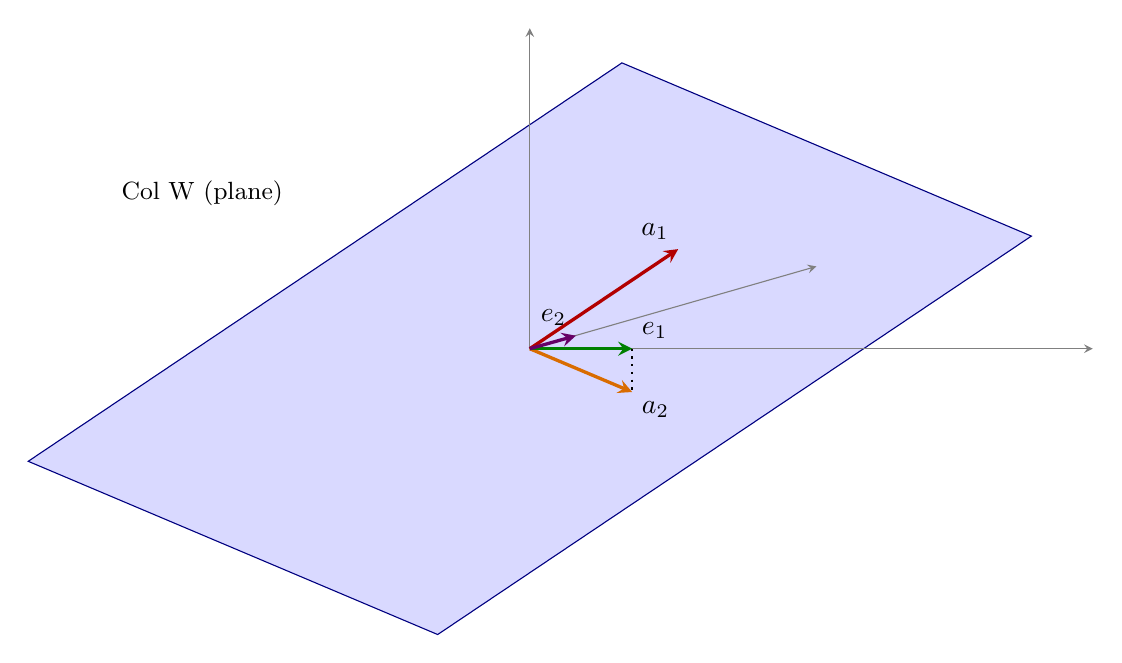
\begin{tikzpicture}[x=1.3cm,y=0.55cm,>=stealth]
  \fill[blue!15,draw=blue!50!black] (4.9,2.6)--(0.9,6.6)--(-4.9,-2.6)--(-0.9,-6.6)--cycle;
  \draw[->,gray] (0,0)--(5.5,0);
  \draw[->,gray] (0,0)--(0,7.4);
  \draw[->,gray] (0,0)--(2.8,1.9);
  \draw[->,very thick,red!70!black] (0,0)--(1.45,2.3);
  \draw[->,very thick,orange!85!black] (0,0)--(1,-1);
  \draw[->,very thick,green!50!black] (0,0)--(1,0);
  \draw[->,very thick,violet!80!black] (0,0)--(0.45,0.3);
  \draw[dotted,thick] (1,0)--(1,-1);
  \node[above left] at (1.45,2.3) {$a_1$};
  \node[below right] at (1,-1) {$a_2$};
  \node[above right] at (1,0) {$e_1$};
  \node[above left] at (0.45,0.3) {$e_2$};
  \node at (-3.2,3.6) {\small Col W (plane)};
\end{tikzpicture}
\end{center}

\textbf{Figure 2.} The plane $\Col W$ (shaded) in $\R^3$, with $\bv{a}_1$, $\bv{a}_2$ in it, and the columns $\bv{e}_1$, $\bv{e}_2$ of the reduced form, which stick out of the plane. The pivot columns of $W$ are a basis for the plane; the pivot columns of the reduced form are not.

\begin{exmp}{One matrix, three bases}{three}
Let $A=\begin{bmatrix}1&0&2&0&-3\\2&1&3&0&-4\\-1&1&-3&1&9\\1&1&1&0&-1\end{bmatrix}$. Find a basis for $\Nul A$, for $\Col A$ and for $\Row A$.

\textbf{Solution.} One row reduction serves all three.
\begin{align*}
\begin{amat}{ccccc}1&0&2&0&-3\\2&1&3&0&-4\\-1&1&-3&1&9\\1&1&1&0&-1\end{amat}
&\rops{R_2-2R_1}
\begin{amat}{ccccc}1&0&2&0&-3\\0&1&-1&0&2\\-1&1&-3&1&9\\1&1&1&0&-1\end{amat}
\rops{R_3+R_1}
\begin{amat}{ccccc}1&0&2&0&-3\\0&1&-1&0&2\\0&1&-1&1&6\\1&1&1&0&-1\end{amat}
\\[4pt]
&\rops{R_4-R_1}
\begin{amat}{ccccc}1&0&2&0&-3\\0&1&-1&0&2\\0&1&-1&1&6\\0&1&-1&0&2\end{amat}
\rops{R_3-R_2}
\begin{amat}{ccccc}1&0&2&0&-3\\0&1&-1&0&2\\0&0&0&1&4\\0&1&-1&0&2\end{amat}
\\[4pt]
&\rops{R_4-R_2}
\begin{amat}{ccccc}1&0&2&0&-3\\0&1&-1&0&2\\0&0&0&1&4\\0&0&0&0&0\end{amat}
\end{align*}
The last matrix is the reduced echelon form $B$. The pivots are in columns $1,2,4$; the free variables are $x_3$ and $x_5$.

\emph{$\Nul A$.} From $B$: $x_1=-2x_3+3x_5$, $x_2=x_3-2x_5$, $x_4=-4x_5$. In parametric vector form
\[
\bv{x}=x_3\begin{bmatrix}-2\\1\\1\\0\\0\end{bmatrix}+x_5\begin{bmatrix}3\\-2\\0\\-4\\1\end{bmatrix},
\]
so $\{(-2,1,1,0,0),\ (3,-2,0,-4,1)\}$ is a basis for $\Nul A\subseteq\R^5$.

\emph{$\Col A$.} Columns $1,2,4$ of $A$: $\{(1,2,-1,1),\ (0,1,1,1),\ (0,0,1,0)\}$ is a basis for $\Col A\subseteq\R^4$. Not the columns of $B$!

\emph{$\Row A$.} The nonzero rows of $B$: $\{(1,0,2,0,-3),\ (0,1,-1,0,2),\ (0,0,0,1,4)\}$ is a basis for $\Row A\subseteq\R^5$.

Notice that the three bases live in different spaces ($\R^5$, $\R^4$, $\R^5$) and have different numbers of vectors. Also $\Col A$ is only a part of $\R^4$: the zero row of $B$ reflects the fact that row~4 of $A$ equals row~2 minus row~1, and every column of $A$ satisfies $b_1-b_2+b_4=0$ (column~3: $2-3+1=0$; see Pause and think~\ref{think:colplane}).
\end{exmp}

\begin{exmp}{A $3\times4$ matrix and its echelon form}{lay}
Let $A=\begin{bmatrix}1&3&0&-2\\2&6&1&1\\1&3&-1&-7\end{bmatrix}$. Find bases for $\Nul A$, $\Col A$ and $\Row A$.

\textbf{Solution.}
\begin{align*}
\begin{amat}{cccc}1&3&0&-2\\2&6&1&1\\1&3&-1&-7\end{amat}
&\rops{R_2-2R_1}
\begin{amat}{cccc}1&3&0&-2\\0&0&1&5\\1&3&-1&-7\end{amat}
\rops{R_3-R_1}
\begin{amat}{cccc}1&3&0&-2\\0&0&1&5\\0&0&-1&-5\end{amat}
\\[4pt]
&\rops{R_3+R_2}
\begin{amat}{cccc}1&3&0&-2\\0&0&1&5\\0&0&0&0\end{amat}
\end{align*}
The echelon form $B$ has pivots in columns $1$ and $3$, and free variables $x_2$, $x_4$ (here $B$ is also reduced).

\emph{$\Col A$:} the pivot columns of $A$, columns $1$ and $3$: $\{(1,2,1),\ (0,1,-1)\}$.

\emph{$\Row A$:} the nonzero rows of $B$: $\{(1,3,0,-2),\ (0,0,1,5)\}$.

\emph{$\Nul A$:} $x_1=-3x_2+2x_4$ and $x_3=-5x_4$, so
$\bv{x}=x_2(-3,1,0,0)+x_4(2,0,-5,1)$, and $\{(-3,1,0,0),\ (2,0,-5,1)\}$ is a basis. Check one vector: $A(2,0,-5,1)=(2-2,\ 4-5+1,\ 2+5-7)=(0,0,0)$.
\end{exmp}

\begin{exmp}{Shrinking the columns of a matrix to a basis}{pivshrink}
The span of the five columns of $A=\begin{bmatrix}1&2&0&3&0\\2&4&1&5&0\\-1&-2&0&-3&1\\-1&-2&-1&-2&0\end{bmatrix}$ is $\Col A$. Which columns can be thrown away?

\textbf{Solution.}
\begin{align*}
\begin{amat}{ccccc}1&2&0&3&0\\2&4&1&5&0\\-1&-2&0&-3&1\\-1&-2&-1&-2&0\end{amat}
&\rops{R_2-2R_1}
\begin{amat}{ccccc}1&2&0&3&0\\0&0&1&-1&0\\-1&-2&0&-3&1\\-1&-2&-1&-2&0\end{amat}
\\[4pt]
&\rops{R_3+R_1}
\begin{amat}{ccccc}1&2&0&3&0\\0&0&1&-1&0\\0&0&0&0&1\\-1&-2&-1&-2&0\end{amat}
\\[4pt]
&\rops{R_4+R_1}
\begin{amat}{ccccc}1&2&0&3&0\\0&0&1&-1&0\\0&0&0&0&1\\0&0&-1&1&0\end{amat}
\\[4pt]
&\rops{R_4+R_2}
\begin{amat}{ccccc}1&2&0&3&0\\0&0&1&-1&0\\0&0&0&0&1\\0&0&0&0&0\end{amat}
\end{align*}
The pivots are in columns $1,3,5$, so $\{\bv{a}_1,\bv{a}_3,\bv{a}_5\}$ is a basis for $\Col A$. The entries of the nonpivot columns of the reduced form give the discarded columns as combinations of the kept ones: $\bv{a}_2=2\bv{a}_1$ and $\bv{a}_4=3\bv{a}_1-\bv{a}_3$. Check the second: $3(1,2,-1,-1)-(0,1,0,-1)=(3,5,-3,-2)$, which is $\bv{a}_4$. This is the Spanning Set Theorem carried out by row reduction: the discarded columns are the ones that are combinations of \emph{preceding} columns (Theorem~\ref{thm:criterion}(b)), and row reduction finds them all at once.
\end{exmp}

\begin{kc}{Three bases for one matrix}{nulcolrow}
Let $A=\begin{bmatrix}1&2&0&1\\0&0&1&3\\1&2&1&4\end{bmatrix}$. (a)~Row reduce $A$ and find a basis for $\Nul A$, one for $\Col A$ and one for $\Row A$. (b)~Let $B$ be the reduced echelon form. Is the set of pivot columns of $B$ contained in $\Col A$? (Hint: what equation do the three entries of every column of $A$ satisfy?) (c)~Why is the set of rows of $A$ itself \emph{not} a basis for $\Row A$?
\end{kc}

\begin{think}{Where does the equation of $\Col A$ come from?}{colplane}
In Example~\ref{ex:three} every column of $A$ satisfies $b_1-b_2+b_4=0$. Row reduce the augmented matrix $[A\ \bv{b}]$ with a general $\bv{b}=(b_1,b_2,b_3,b_4)$, using the same row operations. What is the entry of the last column in the zero row of $B$, and what does Theorem~\ref{4.2-thm:colsub}(c) say about it?
\end{think}

\begin{think}{Rows from $B$, columns from $A$}{rowvscol}
Row operations replace each row of a matrix by a combination of rows. (a)~Why does this make the nonzero rows of $B$ a legitimate choice for a basis of $\Row A$? (b)~Why does the same reasoning fail for columns? Use your answer to explain why we go back to $A$ for $\Col A$.
\end{think}

% ---------------------------------------------------------------------
\subsection*{Bases for subspaces given by a condition}

Many subspaces are not given as $\Nul A$ or $\Col A$ but by an equation or a condition on the entries: ``all $\bv{x}$ with $x_1+x_2+x_3=0$'', ``all polynomials with $p(1)=0$'', ``all symmetric matrices''. The method is always the same: write the general element with its free parameters, split it into one vector for each parameter, and check independence.

\begin{proc}{A basis for a subspace given by a condition}{cond}
\begin{enumerate}
  \item Write the general element of the space (a list of $n$ numbers, a polynomial $a_0+a_1t+\cdots$, a matrix $\begin{bmatrix}a&b\\c&d\end{bmatrix}$) with letters for the entries.
  \item Impose the condition. In $\R^n$ this is a homogeneous linear system: row reduce it and solve for the basic variables. For polynomials and matrices, translate the condition into equations on the coefficients or entries.
  \item Write the general element as a combination $s_1\bv{h}_1+\cdots+s_k\bv{h}_k$ with the free parameters $s_i$ as weights. Then $\Span\{\bv{h}_1,\dots,\bv{h}_k\}$ is the subspace.
  \item Check that $\{\bv{h}_1,\dots,\bv{h}_k\}$ is independent. (If each parameter is the entry/coefficient at its own place, as for free variables, this is automatic.)
\end{enumerate}
\end{proc}

\begin{exmp}{Two equations in $\R^4$}{twoeq}
Let $H_1$ be the set of $\bv{x}$ in $\R^4$ with $x_1+x_2+x_3+x_4=0$ and $x_1-x_3=0$. Then $H_1=\Nul A$ for $A=\begin{bmatrix}1&1&1&1\\1&0&-1&0\end{bmatrix}$ (Theorem~\ref{4.2-thm:nulsub}).
\begin{align*}
\begin{amat}{cccc}1&1&1&1\\1&0&-1&0\end{amat}
&\rops{R_2-R_1}
\begin{amat}{cccc}1&1&1&1\\0&-1&-2&-1\end{amat}
\rops{-R_2}
\begin{amat}{cccc}1&1&1&1\\0&1&2&1\end{amat}
\\[4pt]
&\rops{R_1-R_2}
\begin{amat}{cccc}1&0&-1&0\\0&1&2&1\end{amat}
\end{align*}
Free variables $x_3,x_4$; $x_1=x_3$ and $x_2=-2x_3-x_4$, so $\bv{x}=x_3(1,-2,1,0)+x_4(0,-1,0,1)$ and $\{(1,-2,1,0),\ (0,-1,0,1)\}$ is a basis for $H_1$. Check: $(1,-2,1,0)$ has sum $0$ and $x_1-x_3=0$.
\end{exmp}

\begin{exmp}{A subspace given by parameters}{param2}
Let $H_2=\{(s+2t,\ -s+t,\ 3t,\ s-t):\ s,t\in\R\}$. Writing the general vector as $s(1,-1,0,1)+t(2,1,3,-1)$ shows $H_2=\Span\{(1,-1,0,1),(2,1,3,-1)\}$. The two vectors are not multiples of each other, so they are independent (Theorem~\ref{thm:easy}(c)): a basis for $H_2$. Here the work was done by the description; only independence had to be checked.
\end{exmp}

\begin{exmp}{Polynomials with a root}{rootH}
Let $H_3=\{p\in\mathbb{P}_3:\ p(1)=0\}$. A general $p=a_0+a_1t+a_2t^2+a_3t^3$ has $p(1)=a_0+a_1+a_2+a_3$, so the condition is $a_0=-a_1-a_2-a_3$ and
\[
p=a_1(t-1)+a_2(t^2-1)+a_3(t^3-1).
\]
So $H_3=\Span\{t-1,\ t^2-1,\ t^3-1\}$. These are independent: in $c_1(t-1)+c_2(t^2-1)+c_3(t^3-1)=0$ the coefficient of $t^3$ is $c_3$, of $t^2$ is $c_2$, of $t$ is $c_1$, and all must be $0$. A basis for $H_3$. (Each of the three polynomials has the value $0$ at $t=1$, as it must.)
\end{exmp}

\begin{exmp}{Symmetric matrices}{symm}
A matrix $\begin{bmatrix}a&b\\c&d\end{bmatrix}$ is symmetric when $c=b$. Then
\[
\begin{bmatrix}a&b\\b&d\end{bmatrix}=a\begin{bmatrix}1&0\\0&0\end{bmatrix}+b\begin{bmatrix}0&1\\1&0\end{bmatrix}+d\begin{bmatrix}0&0\\0&1\end{bmatrix},
\]
so the symmetric matrices are the span of $E_{11}$, $E_{12}+E_{21}$, $E_{22}$. The combination is the zero matrix only if $a=b=d=0$: independent. A basis for the subspace of symmetric $2\times2$ matrices.
\end{exmp}

\begin{exmp}{A condition that does not define a subspace}{notsub}
Let $K=\{p\in\mathbb{P}_3:\ p(1)=1\}$. The zero polynomial has value $0$ at $t=1$, so $\bv{0}\notin K$ and $K$ is not a subspace (Theorem~\ref{4.1-thm:subtest}). Since a basis is defined \emph{for a subspace}, the question ``find a basis for $K$'' has no meaning. Compare $H_3$: changing the right-hand side from $0$ to $1$ destroyed the subspace.
\end{exmp}

\begin{kc}{Subspaces given by a condition}{cond}
Find a basis for each subspace. (a)~$\{p\in\mathbb{P}_2:\ p(2)=0\}$. (b)~The $2\times2$ matrices whose diagonal entries add up to $0$. (c)~The plane $x_1-2x_2+3x_3=0$ in $\R^3$.
\end{kc}

\begin{think}{Adding the right-hand side}{affine}
(a)~Is $\{\bv{x}\in\R^3:\ x_1+x_2+x_3=1\}$ a subspace? (b)~Is $\{\bv{x}\in\R^3:\ x_1+x_2+x_3=0\}$? (c)~How does Procedure~\ref{proc:cond} detect the difference?
\end{think}

% ---------------------------------------------------------------------
\subsection*{Two views of a basis}

Definition~\ref{def:basis} asks for two properties at once. Each is the answer to a natural question about a spanning or an independent set, and the two questions turn out to describe the same objects.

\textbf{View 1: a spanning set with nothing to spare.} Let $\mathcal{B}$ span $H$. If $\mathcal{B}$ is dependent, Theorem~\ref{thm:criterion}(a) lets us remove a vector and still span $H$, so something can be taken out. If $\mathcal{B}$ is independent, then no vector can be removed: the vector $\bv{b}_k$ is not a combination of the others, so without it $\bv{b}_k$ is lost from the span. Hence \emph{a basis is a spanning set from which no vector can be removed without shrinking the span}, and conversely a spanning set from which nothing can be removed is independent, hence a basis.

\textbf{View 2: an independent set that cannot grow.} Let $\mathcal{B}$ be independent in $H$. If $\mathcal{B}$ does not span $H$, pick $\bv{v}$ in $H$ outside $\Span\mathcal{B}$. Then $\mathcal{B}$ together with $\bv{v}$ is still independent (Pause and think~\ref{think:outside}); so $\mathcal{B}$ could be enlarged. If $\mathcal{B}$ spans $H$, every $\bv{v}$ in $H$ is a combination of $\mathcal{B}$, and adding it gives a dependent set (Theorem~\ref{thm:criterion}(a)). Hence \emph{a basis is an independent set in $H$ to which no vector of $H$ can be added without destroying independence}.

Shrinking a spanning set (the Spanning Set Theorem) and enlarging an independent set are the two ways of arriving at a basis.

\begin{exmp}{Growing an independent set in $\R^2$}{grow2}
Start with $\{\bv{u}\}$, $\bv{u}=(2,1)$: independent, but its span is only a line. Add $\bv{w}=(1,2)$, which is not on that line: $\{\bv{u},\bv{w}\}$ is independent (not multiples) and spans $\R^2$ (the matrix with these columns has two pivots). It is a basis, and it cannot be enlarged: add any $\bv{z}$, say $\bv{z}=(-1,1)$, and $\bv{z}=\bv{w}-\bv{u}$ is a combination of the others, so $\{\bv{u},\bv{w},\bv{z}\}$ is dependent with relation $\bv{u}-\bv{w}+\bv{z}=\bv{0}$. See Figure 3.
\end{exmp}

\begin{center}
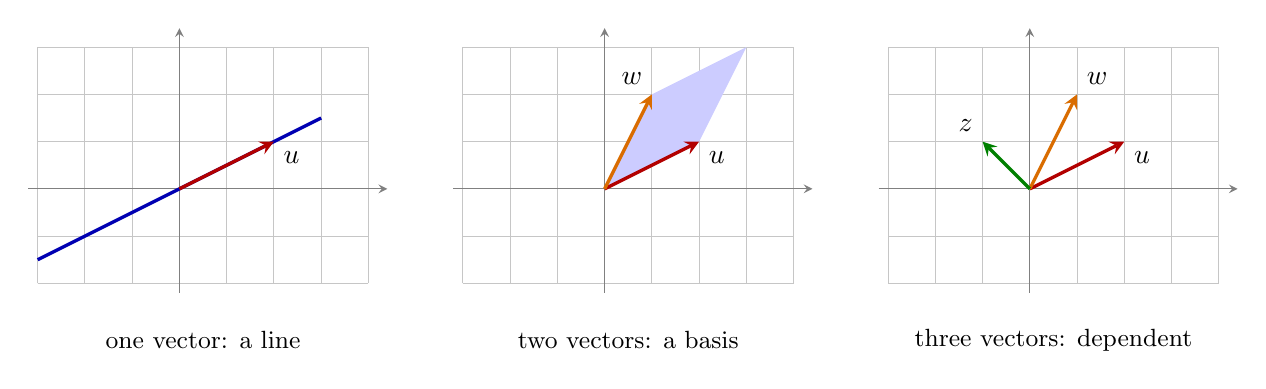
\begin{tikzpicture}[x=0.6cm,y=0.6cm,>=stealth]
  \foreach \sx/\lab in {0/1,9/2,18/3} {
    \begin{scope}[shift={(\sx,0)}]
      \draw[gray!45] (-3,-2) grid[step=1] (4,3);
      \draw[->,gray] (-3.2,0)--(4.4,0);
      \draw[->,gray] (0,-2.2)--(0,3.4);
    \end{scope}
  }
  \draw[very thick,blue!70!black] (-3,-1.5)--(3,1.5);
  \draw[->,very thick,red!70!black] (0,0)--(2,1);
  \node[below right] at (2,1) {$u$};
  \node at (0.5,-3.2) {\small one vector: a line};
  \begin{scope}[shift={(9,0)}]
    \fill[blue!20] (0,0)--(2,1)--(3,3)--(1,2)--cycle;
    \draw[->,very thick,red!70!black] (0,0)--(2,1);
    \draw[->,very thick,orange!85!black] (0,0)--(1,2);
    \node[below right] at (2,1) {$u$};
    \node[above left] at (1,2) {$w$};
    \node at (0.5,-3.2) {\small two vectors: a basis};
  \end{scope}
  \begin{scope}[shift={(18,0)}]
    \draw[->,very thick,red!70!black] (0,0)--(2,1);
    \draw[->,very thick,orange!85!black] (0,0)--(1,2);
    \draw[->,very thick,green!50!black] (0,0)--(-1,1);
    \node[below right] at (2,1) {$u$};
    \node[above right] at (1,2) {$w$};
    \node[above left] at (-1,1) {$z$};
    \node at (0.5,-3.2) {\small three vectors: dependent};
  \end{scope}
\end{tikzpicture}
\end{center}

\textbf{Figure 3.} Left: one vector spans a line, and independence is easy but the span is small. Middle: $\bv{u}$ and $\bv{w}$ together fill the plane. Right: adding $\bv{z}=\bv{w}-\bv{u}$ gives a third vector inside the span of the first two, so the independence is lost.

\begin{exmp}{Growing an independent set in $\R^3$}{grow3}
Start with $\bv{p}_1=(1,1,0)$. Choose $\bv{p}_2=(0,1,1)$, which is not a multiple of $\bv{p}_1$; $\{\bv{p}_1,\bv{p}_2\}$ is independent. Is $\bv{p}_3=(1,0,1)$ in $\Span\{\bv{p}_1,\bv{p}_2\}$? We would need $a(1,1,0)+b(0,1,1)=(a,\ a+b,\ b)=(1,0,1)$, so $a=1$, $b=1$ and $a+b=2\neq0$: impossible. So $\bv{p}_3$ is outside the span and $\{\bv{p}_1,\bv{p}_2,\bv{p}_3\}$ is still independent. It also spans $\R^3$ (three pivots, Example~\ref{ex:isbasis}(a)), so no further vector can be added: any fourth vector is a combination of the first three. We have arrived at a basis for $\R^3$ by growing.
\end{exmp}

\begin{exmp}{Both views agree on a plane}{bothviews}
In Example~\ref{ex:shrink3} the plane $H$ had the spanning set $\{\bv{s}_1,\bv{s}_2,\bv{s}_3,\bv{s}_4\}$ with a vector to spare, and the basis $\{\bv{s}_1,\bv{s}_2\}$. From view 1: remove $\bv{s}_1$ and the span drops, since $\bv{s}_1$ is not a multiple of $\bv{s}_2$; remove $\bv{s}_2$ and the span drops for the same reason. From view 2: any vector of $H$ is already in the span of $\bv{s}_1,\bv{s}_2$, so adding it breaks independence. A vector outside $H$ such as $(1,1,1)$ ($1+1-1=1\neq0$) could be added without destroying independence, but the new set would no longer lie in $H$. The question is always asked \emph{inside} the given subspace.
\end{exmp}

\begin{kc}{The two views}{twoviews}
(a)~Is $\{(1,0,0),(0,1,0),(1,1,0)\}$ a spanning set of $H=\{\bv{x}\in\R^3:\ x_3=0\}$ from which nothing can be removed? (b)~Is $\{(1,0)\}$ an independent set in $\R^2$ to which nothing can be added? (c)~Find an independent set in $\R^3$ with two vectors to which something can be added, and add one.
\end{kc}

\begin{think}{Adding a vector from outside the span}{outside}
Let $\mathcal{B}=\{\bv{b}_1,\dots,\bv{b}_p\}$ be independent and let $\bv{v}$ not be in $\Span\mathcal{B}$. Suppose $c_0\bv{v}+c_1\bv{b}_1+\cdots+c_p\bv{b}_p=\bv{0}$. (a)~Show that $c_0=0$. (Suppose not, and solve for $\bv{v}$.) (b)~Then what do you conclude about $c_1,\dots,c_p$?
\end{think}

% ---------------------------------------------------------------------
\subsection*{Summary}

\begin{itemize}
  \item A set is linearly independent when the only combination giving $\bv{0}$ is the trivial one. Test: put the data (columns, coefficients of $1,t,t^2,\dots$, entries of matrices) into a matrix and look for a pivot in every column; for functions, evaluate at points (this can prove independence only).
  \item A set of two or more vectors is dependent exactly when one of them is a combination of the others; that vector can be removed without changing the span.
  \item A basis for $H$ is an independent set that spans $H$. The standard bases: $\bv{e}_1,\dots,\bv{e}_n$ for $\R^n$; $1,t,\dots,t^n$ for $\mathbb{P}_n$; $E_{11},E_{12},E_{21},E_{22}$ for $M_{2\times2}$.
  \item Spanning Set Theorem: from a spanning set one can remove vectors, one at a time, until a basis remains.
  \item $\Nul A$: free-variable vectors of the parametric vector form. $\Col A$: the pivot columns \emph{of $A$}. $\Row A$: the nonzero rows \emph{of the echelon form}.
  \item For a subspace given by a condition: general element, impose the condition, split by parameters, check independence.
  \item A basis is both a spanning set with nothing removable and an independent set to which nothing can be added.
\end{itemize}

\subsection*{Questions to think about before the next section}

\begin{enumerate}
  \item In Examples~\ref{ex:three} and~\ref{ex:lay} we found bases for $\Nul A$ and $\Col A$ of the same matrix: count the vectors in the two bases of each matrix, and compare the sum with the number of columns of that matrix. What do you notice? Why is it true for the bases we constructed?
  \item Start with the independent set $\{(1,1,1)\}$ in $\R^3$ and enlarge it step by step to a basis for $\R^3$.
  \item Is it possible for a basis of a space to contain the zero vector? Why not?
\end{enumerate}

\subsection*{Answers and discussion}
\begin{description}[leftmargin=0pt,itemsep=5pt]
  \item[Knowledge Check \ref{kc:cols}.] (a)~Row reduce the matrix with these columns:
\begin{align*}
\begin{amat}{ccc}1&2&3\\-1&0&-3\\2&1&4\end{amat}
&\rops{R_2+R_1}
\begin{amat}{ccc}1&2&3\\0&2&0\\2&1&4\end{amat}
\rops{R_3-2R_1}
\begin{amat}{ccc}1&2&3\\0&2&0\\0&-3&-2\end{amat}
\\[4pt]
&\rops{R_3+\tfrac32R_2}
\begin{amat}{ccc}1&2&3\\0&2&0\\0&0&-2\end{amat}
\end{align*}
  Three pivots: independent. (b)~$\begin{bmatrix}1&2\\3&7\end{bmatrix}$ has determinant $7-6=1\neq0$, so two pivots: independent. (c)~The third vector is the sum of the first two, so the set is dependent: $(1,0,1,0)+(0,1,0,1)-(1,1,1,1)=\bv{0}$. (d)~Three vectors in $\R^2$: dependent (Theorem~\ref{1.7-thm:count}); a relation: $(1,2)+(3,1)-(4,3)=(0,0)$.
  \item[Knowledge Check \ref{kc:polymat}.] (a)~The coefficient columns of $2+t$, $1+t^2$, $t+t^2$ are $(2,1,0)$, $(1,0,1)$, $(0,1,1)$:
\begin{align*}
\begin{amat}{ccc}2&1&0\\1&0&1\\0&1&1\end{amat}
&\rops{R_1\leftrightarrow R_2}
\begin{amat}{ccc}1&0&1\\2&1&0\\0&1&1\end{amat}
\rops{R_2-2R_1}
\begin{amat}{ccc}1&0&1\\0&1&-2\\0&1&1\end{amat}
\\[4pt]
&\rops{R_3-R_2}
\begin{amat}{ccc}1&0&1\\0&1&-2\\0&0&3\end{amat}
\end{align*}
  Three pivots: independent. (b)~$(1+t)-(t+t^2)+(t^2+t^3)-(1+t^3)=0$, so the set is dependent. (c)~Call the matrices $N_1,N_2,N_3$. Then $N_1-2N_2-N_3=\begin{bmatrix}1-0-1&2-2-0\\0-2+2&1-2+1\end{bmatrix}=\begin{bmatrix}0&0\\0&0\end{bmatrix}$: dependent.
  \item[Knowledge Check \ref{kc:funcs}.] (a)~If $c_1+c_2e^t=0$ for all $t$: at $t=0$, $c_1+c_2=0$; at $t=1$, $c_1+ec_2=0$. Subtracting: $(e-1)c_2=0$, so $c_2=0$ and $c_1=0$. (b)~At $t=0$: $c_1+c_2=0$. At $t=\tfrac{\pi}{2}$: $0\cdot c_1-c_2=0$, so $c_2=0$ and then $c_1=0$. (c)~At $t=0$ both functions are $0$, so the equation is $0=0$ and says nothing. At $t=\tfrac{\pi}{4}$ the values are $1$ and $\tfrac12$: $c_1+\tfrac12c_2=0$, which has the nonzero solution $(1,-2)$. So the equations are inconclusive (see the warning on evaluating at points). The identity $\sin2t=2\sin t\cos t$ gives $\sin2t-2\sin t\cos t=0$ for all $t$: the set is \emph{dependent}.
  \item[Knowledge Check \ref{kc:removable}.] (a)~$(1,1,0)+(0,1,1)=(1,2,1)$. (b)~$\bv{u}_3$ can be removed. So can $\bv{u}_1$ (since $\bv{u}_1=\bv{u}_3-\bv{u}_2$) and $\bv{u}_2$ (since $\bv{u}_2=\bv{u}_3-\bv{u}_1$), though not several at once. $\bv{u}_4$ cannot: every vector of $\Span\{\bv{u}_1,\bv{u}_2,\bv{u}_3\}=\Span\{\bv{u}_1,\bv{u}_2\}$ has the form $(a,\ a+b,\ b)$, and $(0,0,1)$ would need $a=0$, $a+b=0$, $b=1$: impossible. (c)~Yes: $\bv{u}_1+\bv{u}_2-\bv{u}_3=\bv{0}$ is a dependence relation.
  \item[Knowledge Check \ref{kc:isbasis}.] (a)~Yes: the determinant of $\begin{bmatrix}1&3\\2&5\end{bmatrix}$ is $-1\neq0$, so the vectors are independent and span $\R^2$. (b)~No: they are independent but two vectors cannot span $\R^3$ (at most two pivots, three rows). (c)~Yes: the coefficient columns $(1,0,0)$, $(1,1,0)$, $(2,0,1)$ form an upper triangular matrix with three pivots. (d)~No: $(2,4)=2(1,2)$, so it is dependent (it does span $\R^2$). (e)~No: $(2,4)=2(1,2)$, so it is dependent; $\{(1,2)\}$ alone would be a basis for that line.
  \item[Knowledge Check \ref{kc:shrinkkc}.] (a)~$\bv{v}_2=2\bv{v}_1$ and $\bv{v}_4=\bv{v}_1+\bv{v}_3$ (check: $(1,1,0)+(0,1,1)=(1,2,1)$). (b)~Remove $\bv{v}_2$, then $\bv{v}_4$ (still a combination of what is left). The remaining $\{\bv{v}_1,\bv{v}_3\}$ is independent (not multiples), so it is a basis for $H$. (c)~No. Instead remove $\bv{v}_1=\tfrac12\bv{v}_2$ and $\bv{v}_4$ ($\bv{v}_4=\tfrac12\bv{v}_2+\bv{v}_3$): $\{\bv{v}_2,\bv{v}_3\}$ is also a basis. So is $\{\bv{v}_1,\bv{v}_4\}$.
  \item[Knowledge Check \ref{kc:nulcolrow}.] (a)~Row operations $R_3-R_1$, then $R_3-R_2$ give the reduced form $\begin{bmatrix}1&2&0&1\\0&0&1&3\\0&0&0&0\end{bmatrix}$. Pivot columns $1,3$; free variables $x_2,x_4$ with $x_1=-2x_2-x_4$, $x_3=-3x_4$. Basis for $\Nul A$: $\{(-2,1,0,0),\ (-1,0,-3,1)\}$. Basis for $\Col A$: columns $1,3$ of $A$: $\{(1,0,1),\ (0,1,1)\}$. Basis for $\Row A$: $\{(1,2,0,1),\ (0,0,1,3)\}$. (b)~Every column of $A$ has third entry equal to the sum of the first two, so $\Col A$ lies in the plane $b_3=b_1+b_2$. The pivot columns of $B$ are $(1,0,0)$ and $(0,1,0)$, and $0\neq1$ in both: neither is in $\Col A$. (c)~The third row of $A$ is the sum of the first two: $(1,2,0,1)+(0,0,1,3)=(1,2,1,4)$. The rows are dependent.
  \item[Knowledge Check \ref{kc:cond}.] (a)~$p=a_0+a_1t+a_2t^2$ with $p(2)=a_0+2a_1+4a_2=0$, so $a_0=-2a_1-4a_2$ and $p=a_1(t-2)+a_2(t^2-4)$. Basis $\{t-2,\ t^2-4\}$; independent because of the $t$ and $t^2$ coefficients. (b)~$\begin{bmatrix}a&b\\c&-a\end{bmatrix}=a\begin{bmatrix}1&0\\0&-1\end{bmatrix}+b\begin{bmatrix}0&1\\0&0\end{bmatrix}+c\begin{bmatrix}0&0\\1&0\end{bmatrix}$; these three are independent (the combination is the zero matrix only for $a=b=c=0$), so they are a basis. (c)~$x_1=2x_2-3x_3$, so $\bv{x}=x_2(2,1,0)+x_3(-3,0,1)$. Basis $\{(2,1,0),(-3,0,1)\}$.
  \item[Knowledge Check \ref{kc:twoviews}.] (a)~No: $(1,1,0)=(1,0,0)+(0,1,0)$ can be removed, and the others still span $H$. (b)~No: $(0,1)$ can be added, and $\{(1,0),(0,1)\}$ is still independent. (c)~For example $\{(1,0,0),(0,1,0)\}$; add $(0,0,1)$, which is not in the plane $x_3=0$ spanned by the two.
  \item[Pause and think \ref{think:zerovec}.] (a)~$1\cdot\bv{0}+0\cdot\bv{v}=\bv{0}$ is a dependence relation with a nonzero weight. (b)~Yes: $1\cdot\bv{0}=\bv{0}$. (This is the only one-element set that is dependent.) (c)~A column of zeros has no pivot, so its variable is free: $A\bv{x}=\bv{0}$ has the nonzero solution $\bv{x}=\bv{e}_j$ (the vector with $1$ in the position of the zero column). The columns are dependent, by Theorem~\ref{1.7-thm:cols}.
  \item[Pause and think \ref{think:evalpts}.] (a)~Two points give two equations in three unknowns, and such a system always has a nonzero solution, so two points can never prove independence of three functions. Three points can: at $t=1,2,3$ the matrix is $\begin{bmatrix}1&1&1\\1&2&4\\1&3&9\end{bmatrix}$ with determinant $2\neq0$, so it works as well. (b)~At $t=0$: $c_1+c_2+c_3=0$. At $t=\tfrac{\pi}{2}$: $c_1-c_2+0=0$. These have the nonzero solution $(1,1,-2)$. It does not prove dependence by itself, because two equations in three unknowns always have one. What proves dependence is the identity $1+\cos2t-2\cos^2t=0$ for all $t$; the solution $(1,1,-2)$ merely agrees with it.
  \item[Pause and think \ref{think:order}.] (a)~There are no vectors before $\bv{v}_1$. In Theorem~\ref{thm:criterion}(b) the hypothesis $\bv{v}_1\neq\bv{0}$ rules out the case in which the largest index with a nonzero weight is $j=1$; a dependent set whose reason is $\bv{v}_1$ alone would otherwise give no preceding vector. (b)~Yes, $\{\bv{0},(1,0)\}$ is dependent (it contains $\bv{0}$). But $\bv{v}_2=(1,0)$ is not a combination of $\bv{v}_1=\bv{0}$: every multiple of $\bv{0}$ is $\bv{0}$. So without the hypothesis, part~(b) of the theorem is false.
  \item[Pause and think \ref{think:unique}.] (a)~Because $\mathcal{B}$ spans $H$. (b)~Subtracting gives $(c_1-d_1)\bv{b}_1+\cdots+(c_p-d_p)\bv{b}_p=\bv{0}$; since the basis is linearly independent, every $c_j-d_j=0$. (c)~No. In Example~\ref{ex:polybasis} the weights $5,-8,5$ are the only ones: the argument in (b) shows that two sets of weights must coincide.
  \item[Pause and think \ref{think:manybases}.] (a)~Example~\ref{ex:shrink3}: the bases $\{\bv{s}_1,\bv{s}_2\}$ and $\{\bv{s}_2,\bv{s}_3\}$ have two vectors each. Example~\ref{ex:shrinkpoly}: $\{1,t,t^2\}$ and $\{t,1+t,t^2-t\}$ have three vectors each. (b)~This is a genuine open question for now. Any answer is a guess, and a good guess is supported by testing. Take $\R^2$, which has the basis $\{\bv{e}_1,\bv{e}_2\}$: look for other bases of $\R^2$ using the two definitions (independent, spanning), write down how many vectors each has, and see what your examples suggest. Keep your attempt; we do not settle the matter in this section.
  \item[Pause and think \ref{think:colplane}.] The augmented matrix $[A\ \bv{b}]$ is reduced with the operations $R_2-2R_1$, $R_3+R_1$, $R_4-R_1$, $R_3-R_2$, $R_4-R_2$. The last column becomes $(b_1,\ b_2-2b_1,\ b_3-b_2+3b_1,\ b_4-b_2+b_1)$, and the zero row of $B$ carries the entry $b_1-b_2+b_4$. The system is consistent exactly when this entry is $0$, and by Theorem~\ref{4.2-thm:colsub}(c) $\Col A$ is the set of $\bv{b}$ for which the system is consistent: $\Col A=\{\bv{b}:\ b_1-b_2+b_4=0\}$.
  \item[Pause and think \ref{think:rowvscol}.] (a)~Each row of $B$ is a combination of rows of $A$, so lies in $\Row A$; the nonzero rows span $\Row A$ (Theorem~\ref{4.2-thm:rowops}) and are independent (Theorem~\ref{thm:rowbasis}). (b)~A row operation mixes the entries \emph{within} a column but does not replace columns by combinations of other columns; so the columns of $B$ need not lie in $\Col A$ (Example~\ref{4.2-ex:colchange}). What survives is the set of dependence relations among the columns (the solutions of $A\bv{x}=\bv{0}$), which tells us which columns of $A$ to keep.
  \item[Pause and think \ref{think:affine}.] (a)~No: $\bv{0}$ has sum $0\neq1$. (b)~Yes: it is $\Nul$ of the $1\times3$ matrix $[1\ 1\ 1]$. (c)~Step 2 of the procedure needs a \emph{homogeneous} system (right-hand side $0$) so that the general solution is a combination of vectors with free parameters as weights. With right-hand side $1$ the general solution has an extra constant vector, which cannot be a combination with arbitrary weights.
  \item[Pause and think \ref{think:outside}.] (a)~If $c_0\neq0$, then $\bv{v}=-\tfrac{c_1}{c_0}\bv{b}_1-\cdots-\tfrac{c_p}{c_0}\bv{b}_p$ would lie in $\Span\mathcal{B}$, contrary to the choice of $\bv{v}$. So $c_0=0$. (b)~The equation becomes $c_1\bv{b}_1+\cdots+c_p\bv{b}_p=\bv{0}$, and $\mathcal{B}$ is independent: all $c_i=0$. So the enlarged set is independent.
  \item[Before the next section.] (1)~Example~\ref{ex:three}: $2$ vectors for $\Nul A$ and $3$ for $\Col A$, total $5$, the number of columns. Example~\ref{ex:lay}: $2+2=4$ columns. For the bases we constructed, every column of the matrix is either a pivot column (one vector of the basis for $\Col A$) or a free column (one vector of the basis for $\Nul A$), never both, so the counts add up to the number of columns. (2)~Add $(1,0,0)$: it is not a multiple of $(1,1,1)$, so the pair is independent. The span of the pair consists of the vectors $(a+b,\ a,\ a)$, and $(0,1,0)$ is not of this form ($a=1$ and $a=0$), so it can be added: $\{(1,1,1),(1,0,0),(0,1,0)\}$. The matrix with these columns has determinant $1\neq0$, so it is a basis for $\R^3$. (3)~No: a set that contains $\bv{0}$ is linearly dependent (Theorem~\ref{thm:easy}(b)), so it cannot be a basis.
\end{description}

\end{document}
